% ============================================================================
% THE VALUE-DIRECTED ATTENTION (VDA) SET-SIZE BATTERY.
% Four canonical affine d128 checkpoints: VDA1, VDA2_2x2, VDA4, VDA9.
% Each has one 20,000-row logged phase; this is not a convergence claim.
% All numbers audited against RViT_plus_paper_jepa_grid9/vda_sweep/figs/*.npz.
% Model = affine feedback throughout.
% ============================================================================
\section{The value-directed attention battery: attentional signatures across set size}
\label{sec:vda-battery}

The reproductions above establish that a recurrent vision transformer trained
with reinforcement plus temporal JEPA self-supervision (loss weight $0.5$)
carries the two signal-detection components of attention. We now
ask how those signatures --- and the spatial-cueing, sensitivity, criterion, and
memory effects that accompany them --- depend on the number of competing stimuli.
This is the manipulation that most sharply distinguishes theories of attention:
noise-limited accounts predict that the benefit of attention can \emph{grow} with
set size, because attention may protect the target signal from distractor
noise \cite{carrasco2011_visual_attention_25y}. We compare one canonical affine-feedback
$d_{\mathrm{mem}}=128$ checkpoint at each of four active set sizes: one, two, four,
and nine monitored Gabors (\texttt{vda1}, \texttt{vda2\_2x2}, \texttt{vda4},
\texttt{vda9}). Each checkpoint has a preserved 20{,}000-row metrics phase ending
at logged iteration 19{,}999. This is evidence that the logged phase completed, not
a formal convergence test; resume counters may reset and metrics may be overwritten,
so cumulative lifetime updates are unknown.

The comparison holds the affine-feedback mechanism and memory width in common and uses
related reward and curriculum logic, but it is not an identical-model, identical-task,
or pure-capacity manipulation. VDA1, the canonical VDA2 \texttt{\_2x2} run, and VDA4 use a four-token
$2\times2$ support with different numbers of active cells. VDA9 instead uses a
$3\times3$ grid, nine tokens, a larger image and flattened readout, and training
support that includes an additional $p=0$ condition. The reduced-set-size and base
environments also preserve different validity rules: VDA1 is degenerate; VDA2 uses
\texttt{VDASetSizeEnv} and realizes displayed $p$ exactly; archived VDA4 realizes
$p+(1-p)/4$; and archived VDA9 realizes $p+(1-p)/9$. Thus equal displayed validity
does not guarantee equal realized validity. Learned parameters are separate
at every set size. Thus the four points characterize an association across these
checkpoints; they do not isolate active set size from geometry, token count, readout
dimension, validity semantics, or training support.

The preserved VDA16 phases are incomplete rather than budget-exhausted: their metrics
stop between approximately 622 and 690 logged iterations and their newest checkpoints
are at iteration 599, still near chance at the starting difficulty. They are excluded
from quantitative analysis, and the available files do not reconstruct cumulative
lifetime training.

\begin{quote}\small
\textbf{Frozen legacy-artifact notice (2026-07-07).} The VDA2/VDA9
change-location decode fields and the high-token VDA9 \texttt{crossattn1} clamp
fields are invalid for those claims. The legacy files are preserved unchanged for
provenance; corrected artifacts are pending in a versioned derived path. None of the
claims below relies on those invalid fields.
\end{quote}

Each of the four included checkpoints was subjected to the same battery of
seven analyses: psychometric and chronometric functions, the attention time-course, the
spatial priority map conditioned on cue value and validity, the signal-detection
read-out under a graded attention clamp, the validity (cue-proportion) manipulation, and
temporal decoding of cue validity from working memory. The two remaining analyses of the
core detection battery --- decision-uncertainty read-out and attentional microstimulation
--- were run on the canonical four-stimulus environment and are reported there
(Sections~\ref{sec:det-uncertainty} and \ref{sec:det-microstim}); we do not restate them
per set size.

\subsection{Per-environment deep dives}
\label{sec:vda-perenv}

Figures~\ref{fig:env-vda1}--\ref{fig:env-vda9} report, for each set size, the six
core panels of the battery on one page: (a) the psychometric function (detection vs.\
change magnitude, cued and uncued), (b) the chronometric function (reaction time vs.\
magnitude), (c) the attention time-course (priority on the cued vs.\ other patches
across the seven trial frames), (d) the signal-detection criterion $c$ as the nominal cued-location clamp is swept from suppression to enhancement, (e) the corresponding
sensitivity $d'$, and (f) the validity effect (cued detection threshold vs.\ displayed
cue validity). Every checkpoint is a graded detector and orients attention to the
cued location. Clamp endpoints generally shift criterion in the liberal direction,
but the curves are not uniformly monotone (VDA9 reverses at the high end). The
across-environment \emph{differences} are the subject of Sections~\ref{sec:vda-map}
--\ref{sec:vda-decode}.

\begin{figure}[p]\centering
  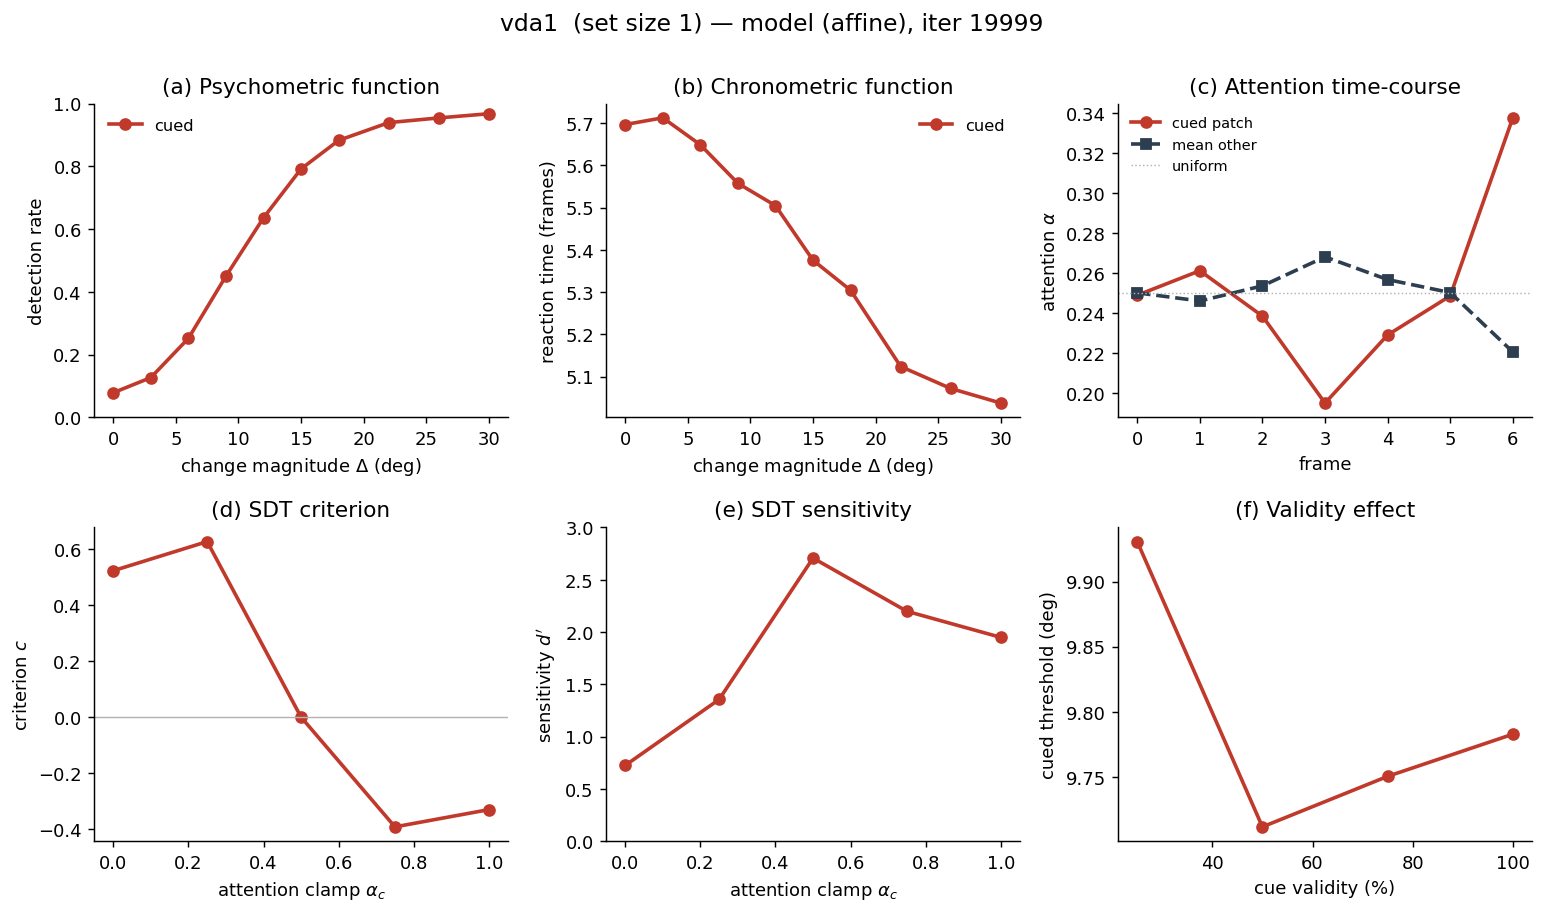
\includegraphics[width=0.95\linewidth]{figures/fig_env_vda1.png}
  \caption{\textbf{Set size 1 (\texttt{vda1}): a single monitored stimulus.} With no
  spatial competition there is no cued/uncued distinction, so the psychometric and
  chronometric functions are cued-only. The mean cued detection threshold is
  $\approx 9.8^\circ$, the lowest of the battery --- detection is easiest when the
  target is alone. The attention clamp produces the \emph{largest} sensitivity
  modulation of any set size ($d'$ swept from $0.72$ to $2.71$), i.e.\ at set size 1
  attention is almost entirely a sensitivity (gain) effect; the criterion also moves
  ($c: 0.52 \to -0.33$).}
  \label{fig:env-vda1}
\end{figure}

\begin{figure}[p]\centering
  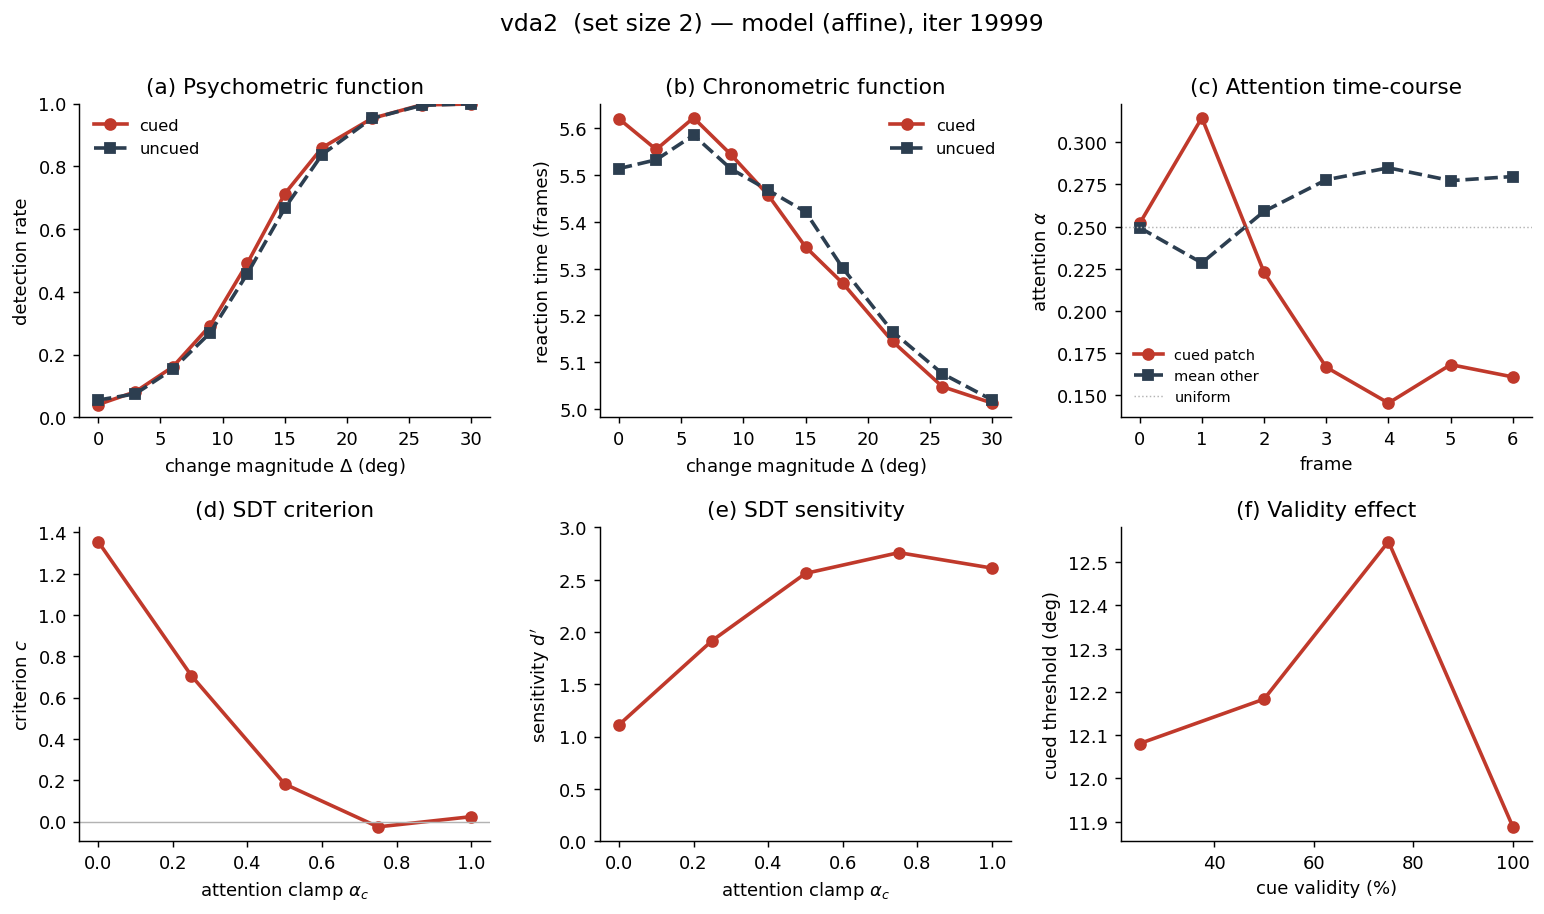
\includegraphics[width=0.95\linewidth]{figures/fig_env_vda2.png}
  \caption{\textbf{Set size 2 (canonical \texttt{vda2\_2x2} checkpoint).} In this
  separately trained task, the cued threshold is $\approx 12.2^\circ$ and panel (a)
  shows a cued-over-uncued benefit. This cross-task contrast does not isolate set size. The
  criterion sweep is the widest of the battery ($c: 1.36 \to 0.02$), while the
  sensitivity modulation begins to compress ($d': 1.11$--$2.76$).}
  \label{fig:env-vda2}
\end{figure}

\begin{figure}[p]\centering
  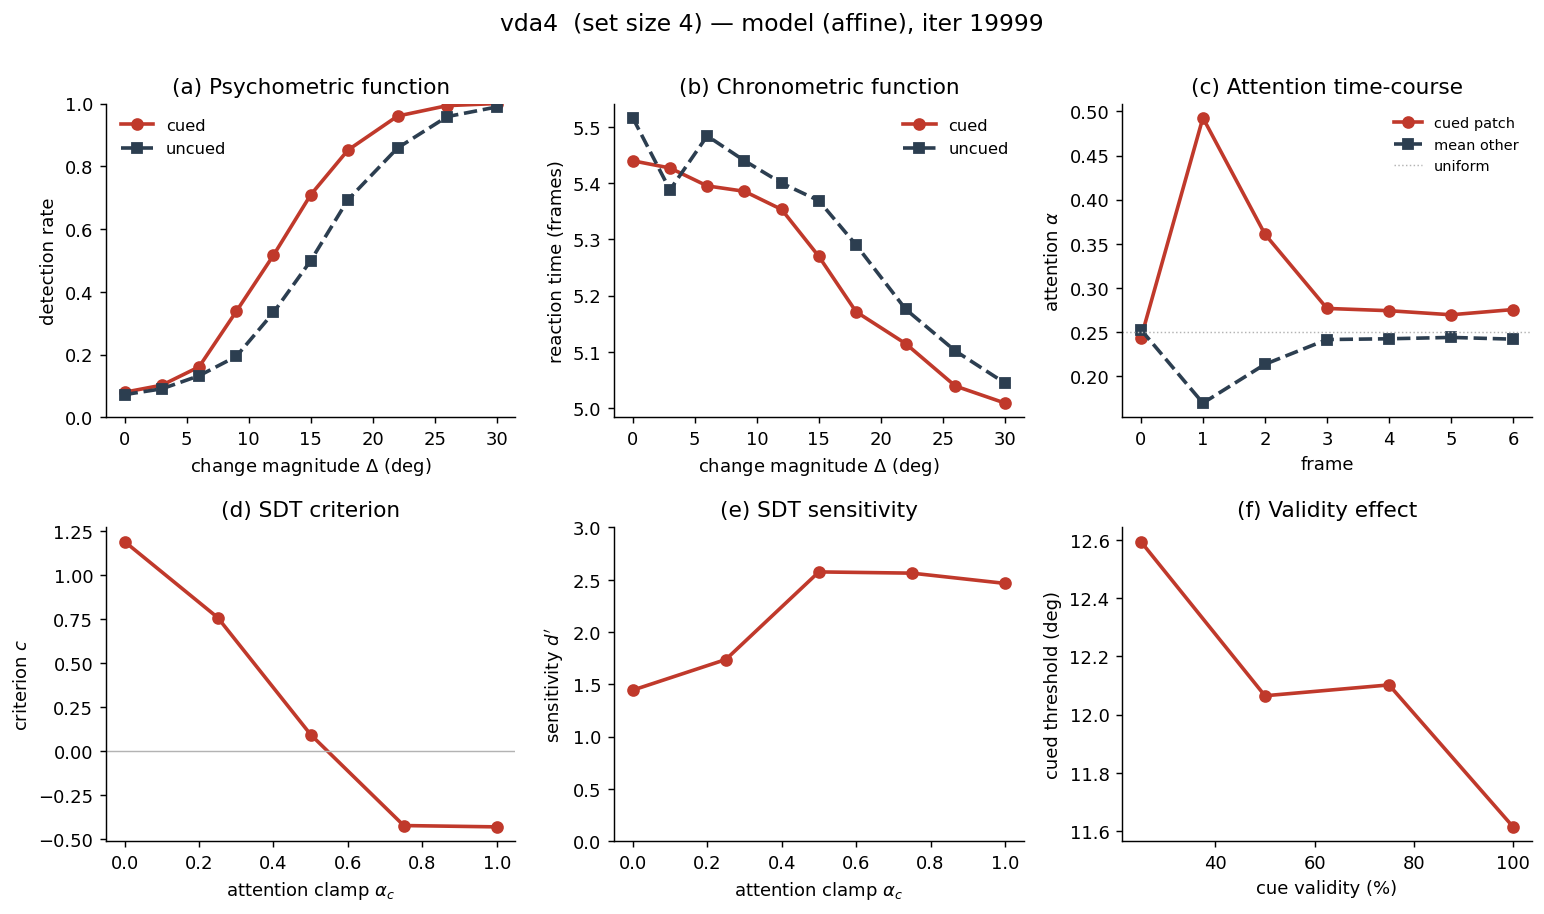
\includegraphics[width=0.95\linewidth]{figures/fig_env_vda4.png}
  \caption{\textbf{Set size 4 (\texttt{vda4}): the canonical published condition.} The
  cued threshold is $\approx 12.1^\circ$; attention lowers the criterion strongly
  ($c: 1.19 \to -0.43$) and still moves sensitivity ($d': 1.44$--$2.57$). The
  attention time-course (panel c) shows the model orienting to the cue and locking onto
  the changed patch, and the map is validity- and value-invariant (Section~\ref{sec:detection}).}
  \label{fig:env-vda4}
\end{figure}

\begin{figure}[p]\centering
  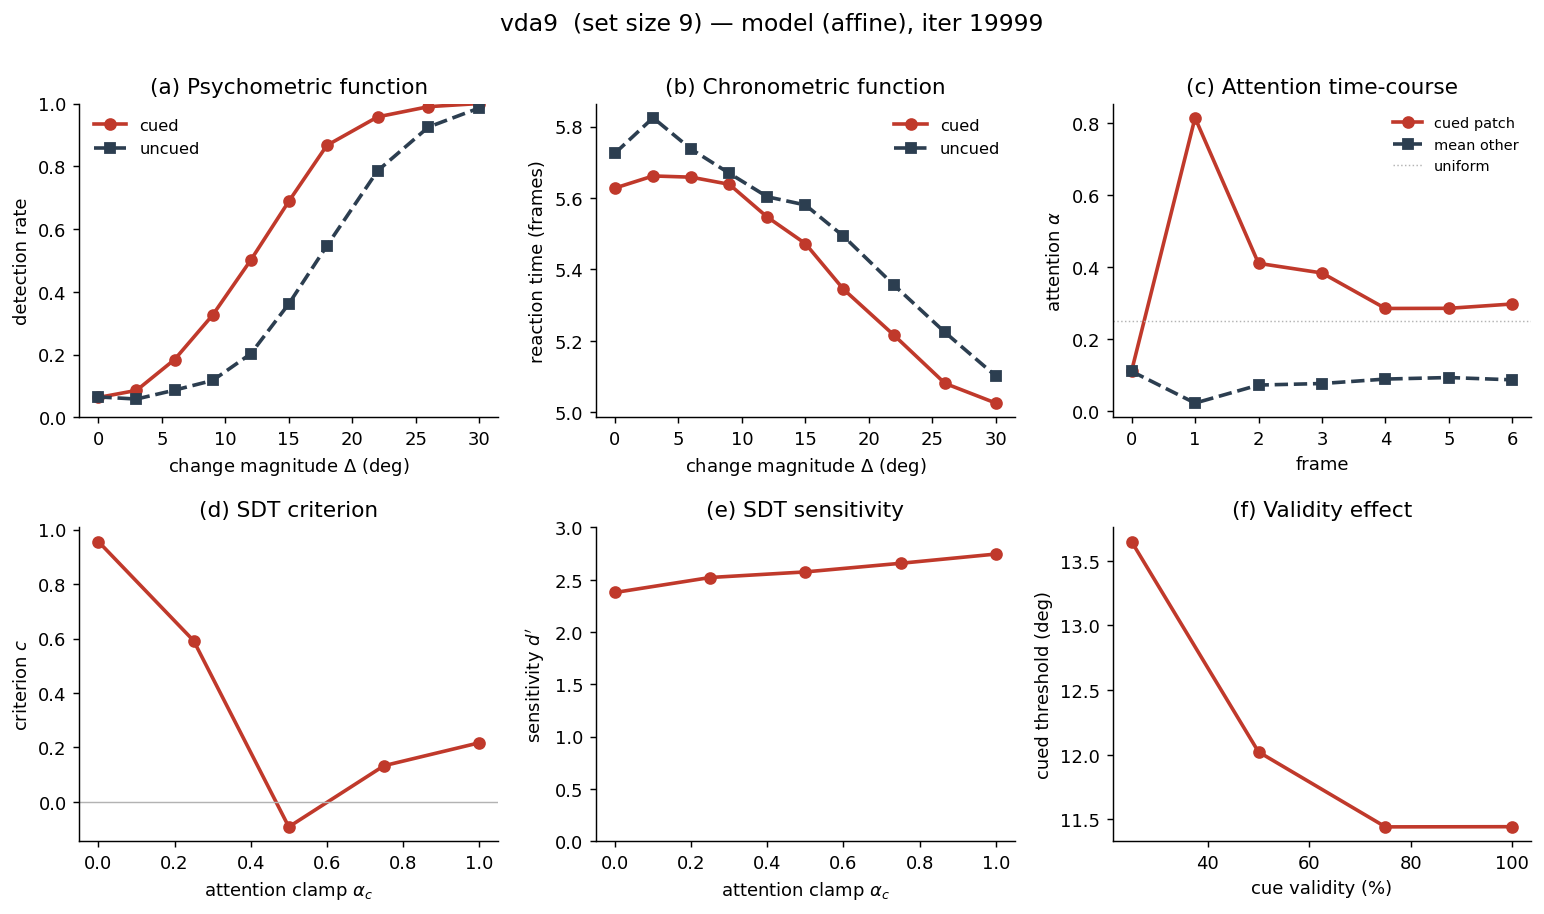
\includegraphics[width=0.95\linewidth]{figures/fig_env_vda9.png}
  \caption{\textbf{Set size 9 (\texttt{vda9}): a $3\times3$ array.} The validity effect
  is now pronounced (panel f: the cued threshold falls steeply as the cue becomes more
  reliable). The nominal attention clamp has the smallest observed sensitivity range
  in the battery ($d': 2.38$--$2.74$). This endpoint range alone does not establish
  saturation or show that sensitivity has ceased to contribute; the criterion range
  is also narrower than at set size 4 ($c: 0.96 \to 0.22$), with a high-clamp reversal
  visible in the full curve.}
  \label{fig:env-vda9}
\end{figure}

\subsection{The priority map: checkpoint-specific orienting with no consistent value steering}
\label{sec:vda-map}

The per-environment panels summarize attention as a single cued-vs-other time-course.
Here we read the model's priority map \emph{spatially}, resolving where attention
falls on each cell of the attention array --- the four cells of the $2\times2$ array for
set sizes 1--4, and all nine cells of the $3\times3$ array for set size 9 --- at each of
the seven trial frames, and asking how that map is shaped by the two cue dimensions the
display carries --- the cue's \emph{value} (its colour: high, mid, or low reward,
red/green/blue) and its \emph{validity} (its ring completeness, $25$--$100\%$).
Throughout, the cued location is the top-left cell, and the uniform baseline is $1/n$ for
an $n$-cell array: $0.25$ for the $2\times2$ set sizes and $0.11$ for the $3\times3$ set
size 9.

\paragraph{Orient at the cue, then release --- largest at cue time in VDA9.}
Figure~\ref{fig:attn-maps} shows the value- and validity-averaged attention map across
the trial for each set size. The common motif is the orient-then-release dynamic
already identified in the core detection analysis (Section~\ref{sec:det-attn}):
attention concentrates on the cued cell at the cue frame ($t_1$) and then relaxes
as the stimulus array is processed. Across these checkpoints, the cue-time
orienting response is largest in VDA9. The peak
cued-cell attention at the cue frame rises from $\approx 0.26$ at set size 1 --- barely
above the $0.25$ uniform, since with a single target there is nothing to orient away from
--- to $\approx 0.81$ at set size 9, where, against a uniform of only $0.11$, the model
throws almost all of its attention onto the cued cell at cue onset ($0.82$ of the total,
versus $\approx 0.02$ on each of the other eight cells) --- the sharpest orienting
transient of the battery. It then settles onto a \emph{sustained} elevation of cued
attention ($\approx 0.31$ through the array frames at set size 9, still nearly three times
its uniform) that is likewise the most pronounced of the ladder. The VDA9 checkpoint therefore shows the largest cue-time concentration, but sustained
attention does not form a strictly monotone four-point ladder. Given the geometry and
training-support changes at VDA9, the pattern is compatible with stronger target
protection under competition but does not by itself establish a noise-limited capacity
law \cite{carrasco2011_visual_attention_25y,%
reynolds_heeger2009_normalization}.

\begin{figure}[t]\centering
  
\includegraphics[width=0.98\linewidth]{figures/fig_attn_maps.png}
  \caption{\textbf{The spatial attention map across the trial, per set size.} Each row
  is one environment; each column is one of the seven trial frames; each panel is the
  attention map in that environment's \emph{native} grid --- $2\times2$ for set sizes
  1--4 and $3\times3$ for set size 9 --- with the cued cell (top-left) outlined in cyan
  (value- and validity-averaged; common colour scale; per-row uniform baseline noted at
  left). Attention concentrates on the cued cell at the cue frame $t_1$ and relaxes
  thereafter; cue-time concentration is largest at set size 9, whereas sustained
  elevation is not strictly monotone across all four checkpoints. At VDA9, $t_1 \approx 0.82$ against
  a uniform baseline of $0.11$ for the nine-cell array, with $\approx 0.02$ on each other
  cell. Separate affine-feedback checkpoints; VDA9 also differs in grid and token/readout dimensions.}
  \label{fig:attn-maps}
\end{figure}

\paragraph{Value does not consistently steer the map in these summaries.}
Conditioning the cued-cell attention on the cue's \emph{value} (Figure~\ref{fig:attn-value-validity},
left) reveals no value-directed steering at any set size. The difference in cued
attention between the highest- and lowest-value cue is small and, critically,
\emph{inconsistent in sign} across the ladder ($+0.05$, $-0.04$, $-0.01$, $-0.08$ at set
sizes $1, 2, 4, 9$): a more valuable cue does not reliably attract more attention, and at
the highest load the lowest-value cue if anything attracts the most. These priority-map
summaries therefore provide no reliable evidence of value-based steering.
This extends the value-invariance observed in the four-stimulus checkpoint
(Section~\ref{sec:det-attn}) to one checkpoint at each included set size. Value is
tracked in memory and can affect decision variables (Section~\ref{sec:value}), while
these priority-map summaries do not show reliable value-based spatial reallocation.

\paragraph{The VDA9 checkpoint shows the strongest validity steering.}
Conditioning instead on cue \emph{validity} (Figure~\ref{fig:attn-value-validity}, right)
shows a strong cross-checkpoint contrast. At set sizes 1, 2, and 4 the cued-cell
attention is essentially flat across displayed validity (the low-to-high-validity change
is $-0.00$, $+0.01$, $+0.01$): the map does not track how reliable the cue is. At set size
9 it steers strongly --- cued attention climbs from $0.33$ at the least-valid cue to $0.47$
at the most-valid cue (a change of $+0.14$), a monotone validity gradient within the VDA9 checkpoint's priority
map. This coincides with stronger validity effects at VDA9 in three readouts:
\emph{behaviour} (a $2.207^\circ$ low-validity minus high-validity \emph{cued-threshold}
improvement, not a cued-versus-uncued spatial benefit; Section~\ref{sec:vda-validity}),
\emph{working memory} (maintained validity decoding, Section~\ref{sec:vda-decode}), and
now the \emph{priority map}. Because this is a cross-checkpoint association with a
concurrent grid and training-support change, it does not establish that load alone
caused this conjunction. It also accords with the isolated-validity environment
(Section~\ref{sec:value-validity4}), where removing the competing value colour lets
validity steer the map ($\alpha_c: 0.27 \to 0.48$) even at moderate load: validity can steer the priority map under at least two separately trained conditions.
The conjunction is compatible with the hypothesis that cue dimensions compete for
retention or control (Section~\ref{sec:value-crowdout}), but these data do not show that
value monopolizes a fixed resource or that validity re-enters at a causal load threshold.

\begin{figure}[t]\centering
  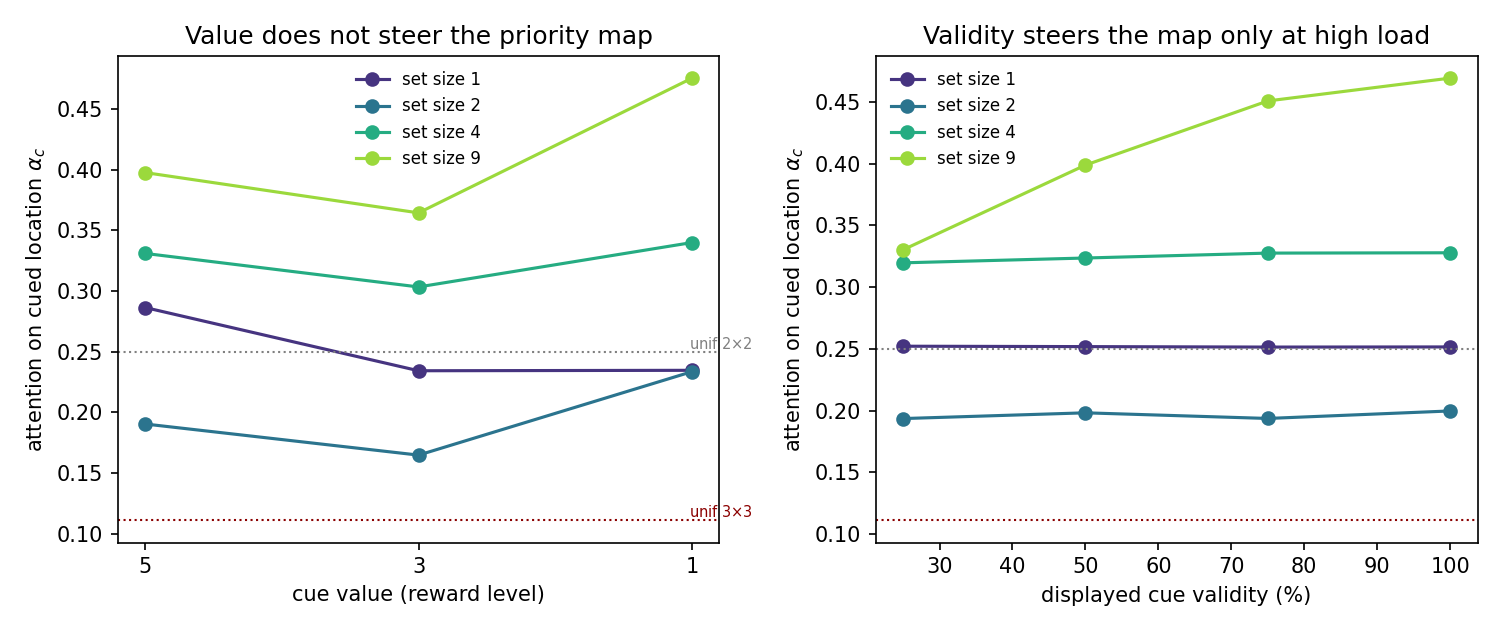
\includegraphics[width=0.95\linewidth]{figures/fig_attn_value_validity.png}
  \caption{\textbf{Priority-map associations with value and validity differ across
  checkpoints.} \emph{Left:} cued-location attention $\alpha_c$ as a function of cue value
  (reward level $5/3/1$), one curve per set size --- small and non-monotone at every set
  size (no value steering). \emph{Right:} $\alpha_c$ as a function of displayed cue
  validity --- nearly flat in VDA1/2/4 and increasing in VDA9. Uniform baselines are
  task-specific: $0.25$ for the $2\times2$ VDA1/2/4 tasks and $1/9\approx0.11$ for
  VDA9. Separate affine-feedback checkpoints; the VDA9 contrast is
  associated with, but does not isolate, load.}
  \label{fig:attn-value-validity}
\end{figure}

\subsection{Validity-threshold changes differ across checkpoints}
\label{sec:vda-validity}

The cued detection threshold changes little across displayed cue validity at set size 1
and more strongly in the VDA9 checkpoint (Figure~\ref{fig:validity-setsize}). Defined
specifically as \emph{low-validity minus high-validity cued threshold}, the four
improvements are $0.148^\circ$, $0.193^\circ$, $0.979^\circ$, and $2.207^\circ$ for
VDA1, VDA2, VDA4, and VDA9. The $2.207^\circ$ quantity is therefore not a spatial
cued-versus-uncued benefit. The ordered increase is consistent with greater use of a
predictive cue as competition increases \cite{carrasco2011_visual_attention_25y}, but
the single-checkpoint design and the VDA9 geometry, readout, validity-semantic, and
training-support differences prevent interpreting it as a pure capacity law. It also qualifies
an apparent paradox in the single-environment analysis (Section~\ref{sec:detection}),
where validity looked ``inert'': the four-stimulus checkpoint has a modest threshold
association that is easier to see in the cross-checkpoint summary.

\begin{figure}[t]\centering
  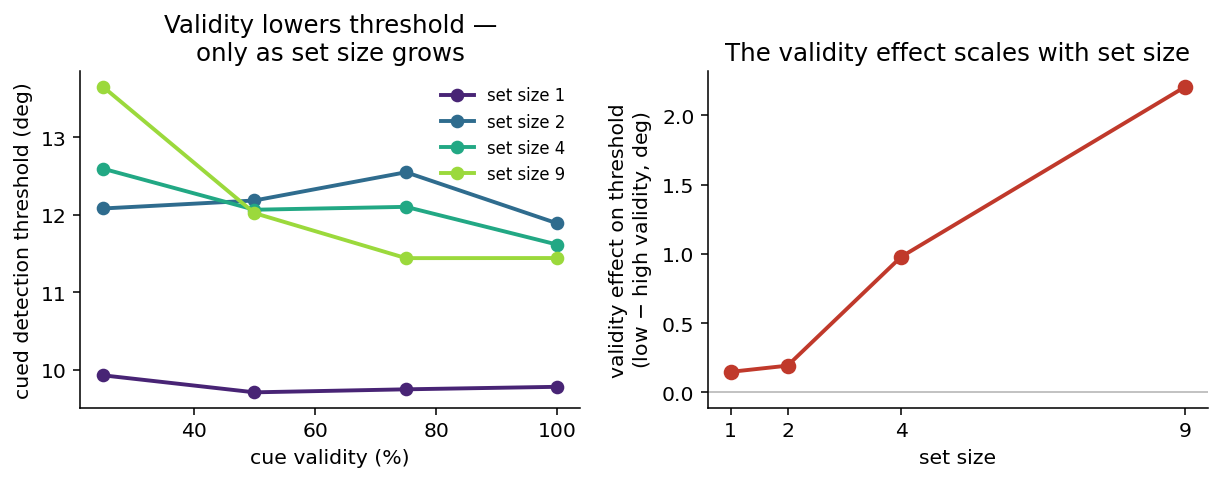
\includegraphics[width=0.95\linewidth]{figures/fig_validity_by_setsize.png}
  \caption{\textbf{Low-to-high-validity cued-threshold changes across checkpoints.} \emph{Left:} cued
  detection threshold vs.\ displayed cue validity, one curve per set size --- flat at
  VDA1, steeply decreasing in VDA9. \emph{Right:} the displayed-validity
 effect is defined as low-validity minus high-validity \emph{cued} threshold and is
 $0.148^\circ$, $0.193^\circ$, $0.979^\circ$, and $2.207^\circ$; it is not a
 cued-versus-uncued benefit. Separate affine-feedback checkpoints.}
  \label{fig:validity-setsize}
\end{figure}

\subsection{Clamp-induced criterion and sensitivity ranges differ across checkpoints}
\label{sec:vda-sdt}

Sweeping the nominal cued-location clamp and reading out signal-detection quantities at
each set size (Figure~\ref{fig:sdt-setsize}) yields two patterns that must be kept
separate from the validity-threshold improvements above. For each quantity we report
its maximum minus minimum over the clamp sweep. The sensitivity ranges are $1.982$,
$1.647$, $1.131$, and $0.367$ for VDA1, VDA2, VDA4, and VDA9. The criterion ranges are
$1.020$, $1.381$, $1.622$, and $1.048$. Thus sensitivity range decreases across these
four checkpoints, whereas criterion range is non-monotone and largest at VDA4. The
small VDA9 $d'$ range does not demonstrate physiological saturation or the absence of a
sensitivity contribution; it is an observed clamp range from one checkpoint. Moreover,
the VDA9 criterion curve reverses at the high-clamp end, so a blanket monotonic-criterion
description is inaccurate.

Because $d'$ range, criterion range, and low-to-high-validity threshold improvement are
different outcomes, we do not combine them into one scalar ``attentional benefit'' or
capacity law. Their differing profiles instead motivate a controlled replication that
holds grid, tokens, readout, validity semantics, and training support fixed. The present
results establish descriptive, checkpoint-specific load associations and a causal
within-checkpoint clamp response, not a single mechanism that changes monotonically
with set size.

\begin{figure}[t]\centering
  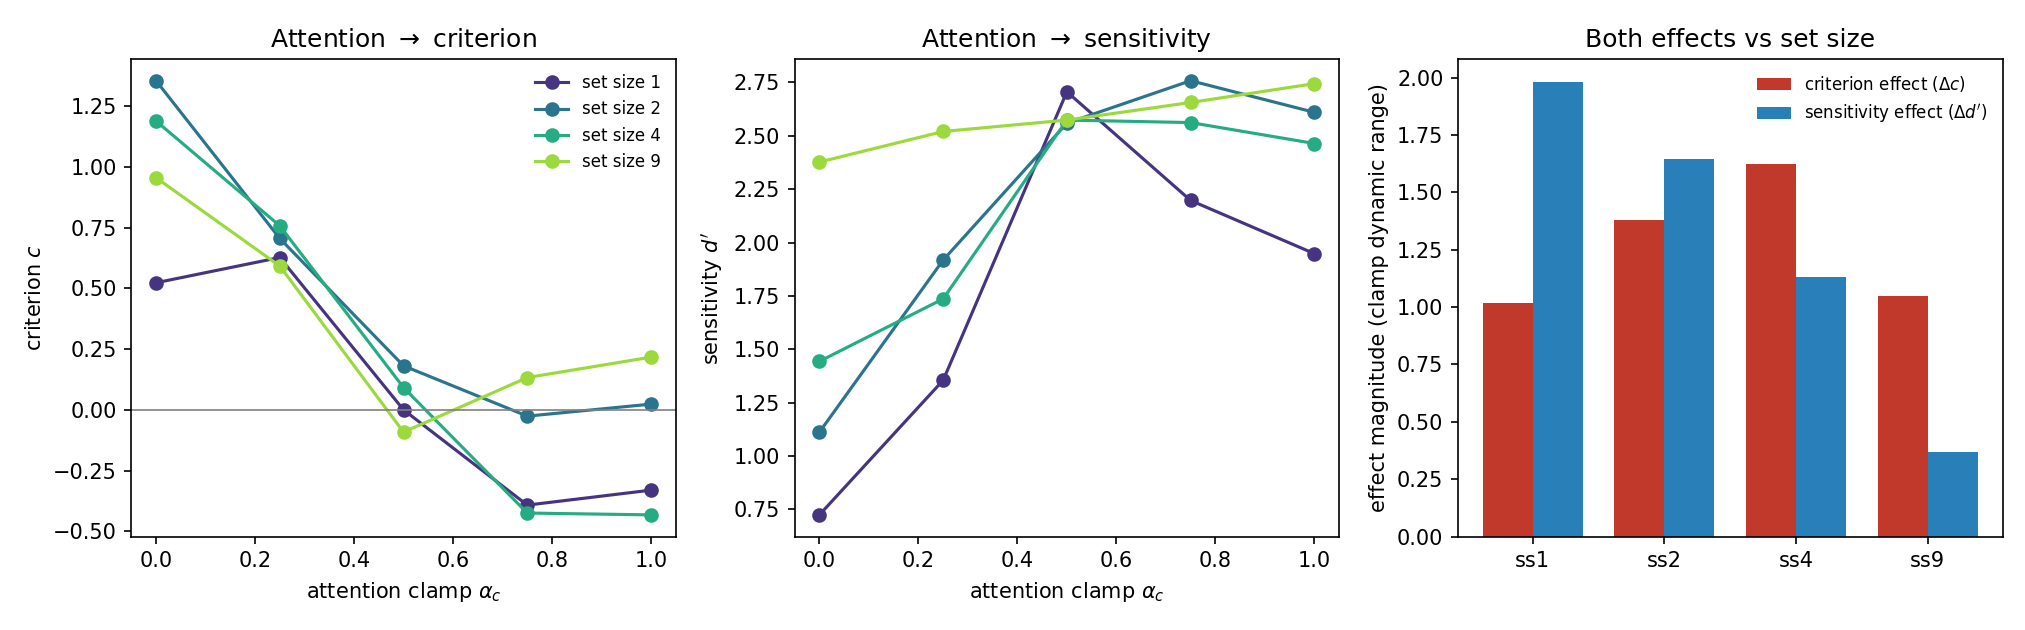
\includegraphics[width=0.98\linewidth]{figures/fig_sdt_by_setsize.png}
  \caption{\textbf{Criterion and sensitivity across set size.} \emph{Left:} criterion
  $c$ vs.\ the attention clamp, one curve per set size. \emph{Middle:} sensitivity $d'$
  vs.\ the clamp. \emph{Right:} the magnitude of each effect (clamp range) against set
  size. Sensitivity ranges are $1.982$, $1.647$, $1.131$, and $0.367$; criterion
  ranges are $1.020$, $1.381$, $1.622$, and $1.048$. These are clamp ranges, not the
  displayed-validity threshold improvements. VDA9 criterion is not uniformly monotone.}
  \label{fig:sdt-setsize}
\end{figure}

\subsection{Validity decoding from working memory differs across checkpoints}
\label{sec:vda-decode}

Finally we ask whether the \emph{maintenance} of cue validity in working memory ---
not just its behavioural expression --- depends on set size. Decoding the displayed cue
validity from the recurrent memory state at each frame (balanced accuracy, held-out
four-way logistic probe; chance $=0.25$) tests whether the model perceives and holds the
cue's reliability (Figure~\ref{fig:decode-setsize}). The result is strongest at VDA9 but is not a monotone ladder at the intermediate
checkpoints. At set size 1, validity is barely encoded even at the cue frame (peak
$0.35$) and is at chance thereafter --- the model does not hold a cue reliability that
cannot help it. At set sizes 2 and 4, validity is strongly perceived at the cue (peak
$0.85$ and $0.77$) but becomes only weakly linearly recoverable within a frame or two
(mean post-cue accuracy $0.35$ and $0.31$, near chance) --- the cue-locked pattern reported for
the single four-stimulus environment (Section~\ref{sec:detection}). In VDA9,
however, the validity-decoding point estimate is $1.00$ at the cue and
is \emph{maintained across the entire trial} (mean post-cue accuracy $0.70$, still
$0.51$ at the final frame). The mean post-cue balanced accuracies for VDA1, VDA2,
VDA4, and VDA9 are approximately $0.247$, $0.350$, $0.309$, and $0.701$:
VDA9 is clearly highest, while VDA2 and VDA4 do not order monotonically.

The contrast with the \emph{value} signal on the same cue is stark and completes the
account. Decoding the cue's value (its colour) from the identical memory state yields a
approximately $1.00$ at the cue frame and subsequent sampled frames in every included
checkpoint (Figure~\ref{fig:decode-setsize}, dashed). Value is thus linearly recoverable
at ceiling in these evaluations; validity is encoded well but
released within a frame or two unless the load is high. The two cue dimensions therefore
receive different treatment in these checkpoints: value is retained at ceiling, whereas
validity is retained most strongly in VDA9. This pattern is compatible with the proposed
cue-competition account (Section~\ref{sec:value-crowdout}) and accompanies the VDA9
validity-steered priority map (Section~\ref{sec:vda-map}); it does not establish value
monopolization or a fixed representational share.

This is a memory-level counterpart of the behavioural VDA9 contrast
(Section~\ref{sec:vda-validity}): the VDA9 checkpoint retains cue reliability more
strongly than the other canonical checkpoints. Whether active load makes that
reliability worth holding is a hypothesis for a fixed-geometry, replicated intervention,
not a functional result established by the present cross-checkpoint comparison. The
pattern is nevertheless consistent with task-relevance-gated encoding described for
prefrontal working memory
\cite{awh_vogel_oh2006,awh_jonides2001_overlapping_attention_wm}.

\begin{figure}[t]\centering
  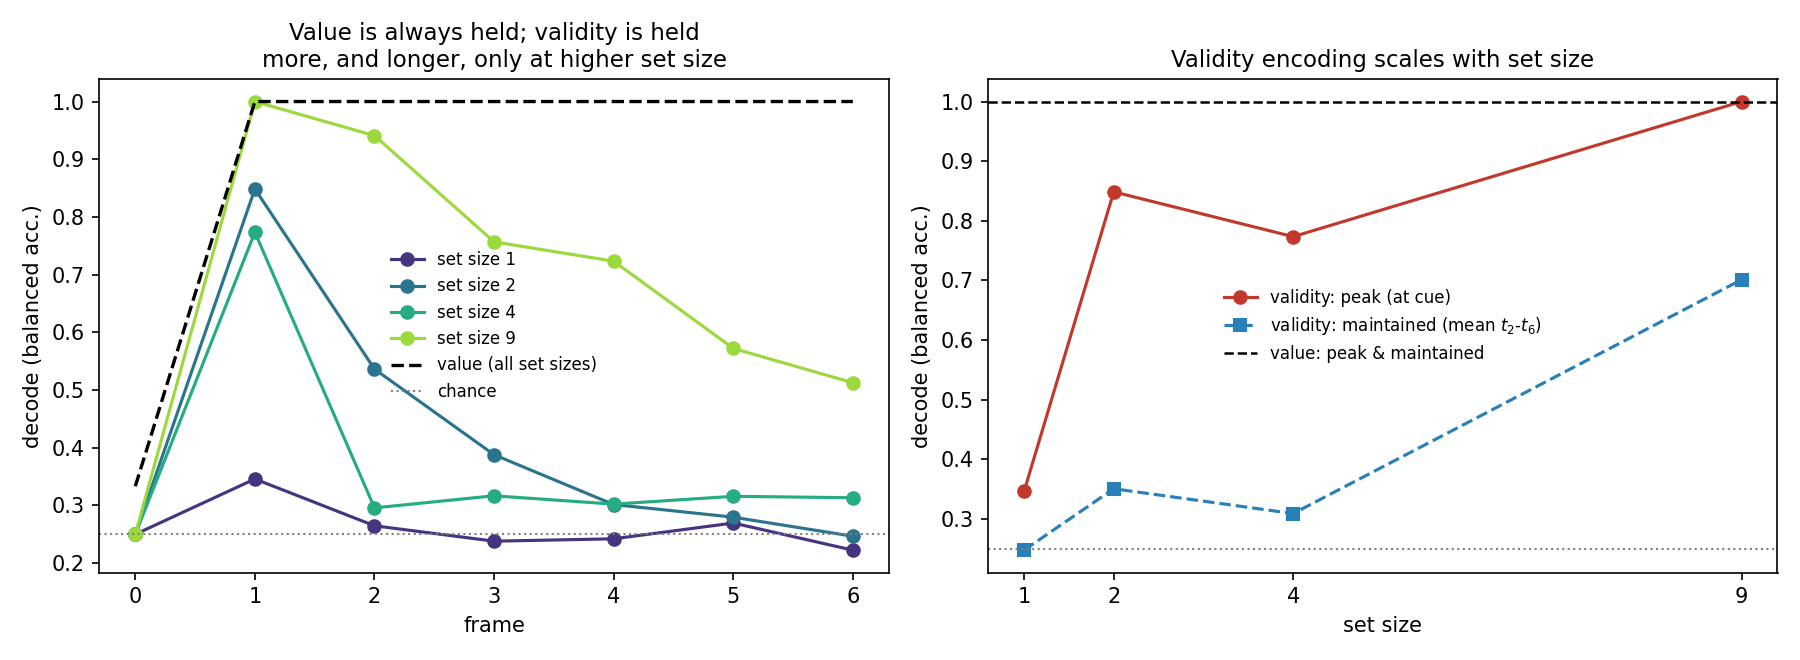
\includegraphics[width=0.95\linewidth]{figures/fig_decode_by_setsize.png}
  \caption{\textbf{Validity-decoding profiles differ across checkpoints, while value
  remains recoverable at ceiling.} \emph{Left:} balanced accuracy of decoding displayed cue
  validity from the recurrent memory state, per frame, one solid curve per set size
  (chance $0.25$); the dashed black line is the value (cue-colour) decode, pinned at
  $\approx 1.0$ across all set sizes. Validity decays after the cue except at set size 9;
  the value decode remains near ceiling. \emph{Right:} the peak (at-cue) and maintained (mean over post-cue
  frames) validity decoding is highest at VDA9 but not monotone at the intermediate
  checkpoints, whereas value (dashed) is at ceiling for peak and maintained at every
  set size. Separate affine-feedback checkpoints.}
  \label{fig:decode-setsize}
\end{figure}
